\chapter{Experimentos}
\label{cap:comprovacao}

Neste capítulo são abordados os testes e experimentos realizados, visando demonstrar o funcionamento da abstração Net Topo e avaliar sua escalabilidade.
A Seção~\ref{sec:testes} apresenta a metodologia de testes utilizada e as funcionalidades cobertas pelos testes.
Na Seção~\ref{sec:my_lb} é descrito um balanceador de carga e a sua modificação, utilizados para comparação.
Na Seção~\ref{sec:overhead} é observado o sobrecusto da abstração comparado um balanceador com a abstração nativa do \charm com o mesmo balanceador mas com a Net Topo.
Por último, são apresentadas os tempo de execução de algumas das funções da abstração e a escalabilidade delas na Seção~\ref{sec:bench}.
% o que vai ter nesse capitulo
% porque desse capítulo


\section{Testes de Funcionamento}
\label{sec:testes}

% Moral dos testes
% Como foram feitos
% O que testam
% qual as limitações dos testes

A comprovação do funcionamento da Net Topo foi feito com a utilização de testes de unidade sob topologias manualmente inicializadas.
Foram implementados 132 testes para cobrir o funcionamento adequado dos métodos e seus componentes, garantindo seu funcionamento independente de sua forma de inicialização.
Foi confeccionado um teste para cada tipo de modificação e retorno previstos nas funcionalidades, como valores nos limites da memória.
Por exemplo, na inserção da estrutura de matriz reflexiva e sem diagonais, foi testado uma inserção comum, uma em cada extremidade da matriz, uma em diagonal, uma reflexiva e uma inválida.

\begin{figure}[h]
\begin{subfigure}{.5\textwidth}
    \centering
    \includegraphics[width=0.8\linewidth]{images/testes_topo_uneven.pdf}
    \caption{Topologia simétrica com um \textit{link} custoso.}
    \label{fig:tested_topologies:small}
\end{subfigure}
\begin{subfigure}{.5\textwidth}
    \centering
    \includegraphics[width=0.8\linewidth]{images/testes_real_topo_no_links.pdf}
    \caption{Topologia assimétrica. \textit{Links} azuis, verdes e vermelhas têm custo 1, 2 e 8, respectivamente.}
    \label{fig:tested_topologies:real}
\end{subfigure}
\caption[Topologias utilizadas para teste.]{Topologias utilizadas para teste.}
\label{fig:tested_topologies}
\end{figure}

A Figura~\ref{fig:tested_topologies} apresenta duas topologias utilizadas para testar as funcionalidades da abstração.
Como a inicialização das topologias foi manual, não foram utilizadas topologias muito grandes.
A topologia (a) tem como objetivo verificar o funcionamento correto dos métodos de distância e \hops.
A topologia (b) apresenta um ambiente heterogêneo e um maior detalhamento da estrutura interna de cada máquina, permitindo observar a divisão adequada entre topologia de máquina e de rede feita pela abstração.
Para avaliar um funcionamento mais extenso na topologia de rede, a topologia (b) é utilizada novamente considerando cada PE como uma máquina individual.

As funcionalidades cobertas pelos testes são: (1) número de PEs na topologia; (2) número de máquinas na topologia; (3) PEs de uma máquina; (4) máquina de um determinado PE; (5) nó de um determinado PE; (6) outros PEs na máquina de um determinado PE; (7) PEs em uma determinada máquina; (8) outros PEs no mesmo nó de um determinado PE; (9) PEs em um determinado nó; (10) número de \links na camada de rede; (11) nome da topologia; (12) mudança de nome da topologia; (13) vizinhos na camada de rede; (14) proximidade entre dois PEs; (15) distância mínima entre dois PEs; (16) \textit{hops} entre dois PEs; (17) serialização de uma topologia; (18) leitura de uma topologia; (19) inicialização de uma topologia; e (20) persistência de informações entre execuções.

Em relação às estruturas utilizadas foram cobertas as seguintes funcionalidades: (1) criação de um CSC com um mecanismo de memoização; (2) inserção em um CSC; serialização de um CSC; (3) cálculo de distância mínima em um CSC; (4) utilização da memoização no cálculo de distâncias do CSC; (5) criação de uma matriz triangular superior sem diagonal; (6) inserção em uma matriz triangular superior sem diagonal; e (7) serialização de uma matriz triangular superior sem diagonal.

%Para garantir que não há escapamento de memória ou leituras invalidas, foi utilizada a ferramenta \textit{valgrind}.

\section{Balanceador de Carga}
\label{sec:my_lb}

% Porque usar um balanceador de carga
% porque usar este balanceador de carga
% O que faz esse balanceador
% o que foi modificado nesse balanceador

Para a demonstração do funcionamento da abstração da topologia de rede, foi modificado um balanceador de carga distribuído presente na plataforma \charm, de nome NeighborLB.
A modificação realizada só alterou de onde as informações de topologia foram retiradas, substituindo a implementação nativa pela Net Topo, sendo que o algoritmo do balanceador não foi alterado.
Este balanceador observa somente PEs vizinhos para a tomada de decisão de balanceamento, evitando contenção da rede e obtendo baixa latência nas mensagens.
Assim como outros balanceadores distribuídos, o NeighborLB  é escalável, pois independe do número de nós da rede. Porém, seu balanceamento é limitado pela quantidade de informação.

O descobrimento de vizinhos no balanceador NeighborLB é dado através de um balanceador base que existe dentro da plataforma \charm que utiliza seu mecanismo de inferência.
Este mecanismo foi substituído pela abstração criada para comprovar seu funcionamento.

A escolha do balanceador NeighborLB se deu pela sua simplicidade e por observar somente seus vizinhos, criando um cenário de comparação equivalente para a abstração Net Topo.
Os métodos de cálculo de \hops do \charm são mais velozes por considerarem topologias especificas (e as vezes imprecisas), o que causaria um cenário onde não se poderia avaliar o sobrecusto da abstração de maneira equivalente.
Nenhum dos balanceadores que utiliza as informações topológicas do \charm possui um cálculo de distância, por não possuir nenhuma informação de latência, inviabilizando a comparação neste nível.
% avaliam um unico core, de uma unica maquina, comparando diferentes topologias para ver como trabalha em escalas diferentes. Pode ter uso 

%mas eu vou tirar informação do charm pra por de novo? > facilidade no acesso, sem ter de realizar de novo


\section{Avaliação de Sobrecusto}
\label{sec:overhead}

% Porque avaliar o sobrecusto
% Como que foi feita essa avaliação

Para observar o sobrecusto da abstração, foi comparada a execução do balanceador NeighborLB, detalhado na Seção~\ref{sec:my_lb}, com o balanceador myNeighborLB, uma modificação do anterior que utiliza a Net Topo em vez do sistema topológico do \charm.
O objetivo da comparação é observar se há uma discrepância de desempenho no uso da abstração, verificar o uso funcional das abstração junto ao modulo de balanceamento de carga do \charm e observar possíveis ganhos e perdas de desempenho da abstração.

O \textit{benchmark} sintético \textit{LB Test} foi utilizado para realizar uma avaliação da execução dos balanceadores de carga.
Nele são criadas cargas uniformemente distribuídas entre uma valor de carga mínimo e máximo. 
O \textit{LB test} cria um perfil de comunicação entre estas cargas e invoca um balanceador de carga periodicamente, ambos escolhidos pelo usuário.
As configurações do \textit{LB test} são abordadas na Subseção~\ref{subsec:casos_exec}.
O ambiente de execução do \textit{benchmark }é determinado por um arquivo de grupos de execução, contendo as máquinas que serão utilizadas e seus IPs.
No caso deste trabalho, as máquinas Ciclope e Centauro foram utilizadas, detalhadas a seguir.

\subsection{Ambiente de Execução}
\label{subsec:ambiente}

% Onde é executado

A execução foi realizada em um conjunto de duas máquinas diferentes: (i) Ciclope e (ii) Centauro.
A primeira máquina utiliza 4 CPUs Intel Core i7-7700 @3.60GHZ com \textit{hypertreading} e possui 8GB@1200 MHz de memória. Possui 3 níveis de cache com tamanhos de 32 KB, 256 KB e 8 MB.
Sua versão de GCC é 5.5.0.
A segunda máquina possui 4 CPUs Intel Core i5-7400 @3.00GHz e 16GB@2400 MHz DIMM de memória. Possui 3 níveis de cache com tamanhos de 32 KB, 256 KB e 6 MB. GCC instalado na versão 5.4.0.
Ambas as máquinas utilizam Linux Mint na versão 18.2 e \charm 6.9.0.
A Figura~\ref{fig:run_topology} apresenta a topologia de cada máquina e do ambiente como um todo. 


\begin{figure}[h]
\begin{subfigure}{.6\textwidth}
    \centering
    \includegraphics[width=0.8\linewidth]{images/init_real_topo.pdf}
    \caption{Em vermelho os agrupamento das máquinas Centauro (A) e Ciclope (B). Em verde os agrupamentos de \textit{cache}.}
    \label{fig:exec:machine_topos}
\end{subfigure}
\begin{subfigure}{.4\textwidth}
    \centering
    \includegraphics[width=0.8\linewidth]{images/execucao_topo.pdf}
    \caption{Topologia de rede do ambiente. Círculos azuis representam os PEs da máquina Ciclope e em laranjas os da máquina Centauro.}
    \label{fig:exec:full_topos}
\end{subfigure}
\caption[Topologia das máquinas Ciclope e Centauro.]{Topologia do ambiente de execução. Os agrupamentos de cada máquina  estão em (a) e a topologia de rede em (b).}
\label{fig:run_topology}
\end{figure}

\subsection{Casos de Execução}
\label{subsec:casos_exec}
% Quais testes vão ocorrer
% Como que os testes vão ocorrer
% Como foram realizados
% O que medem

Foram realizados três configurações do \textit{LB test} para realizar os experimentos capturados neste trabalho, com os seguintes nomes: (i) \textit{init}, (ii) \textit{LB test M} e (iii) \textit{LB test G}.
A Tabela~\ref{tab:execution_count} apresenta o nome de cada configuração e o número de execuções de cada uma delas.
A primeira configuração visa observar os tempos de inicialização da abstração de topologia Net Topo, do armazenamento dela, da inicialização da topologia nativa do \charm e da inicialização através de um arquivo XML. 
Portanto, não é preciso executar nenhum balanceamento de carga e o \textit{LB test} foi utilizado por conveniência.
As configurações (ii) e (iii) visam observar variação no desempenho do balanceador.
Em ambas foi utilizada uma execução de 150 iterações com o balanceador sendo invocado a cada 40 iterações, o intervalo de carga foi de 30 a 4120ms e o padrão de comunicação utilizado foi de anel.
A diferença entre as configurações (ii) e (iii) é o número de tarefas criadas.
Na configuração \textit{LB test M} foram criadas 3600 tarefas (300 tarefas por PE) enquanto na configuração \textit{LB test G} este número foi aumentado para 5400 (450 tarefas por PE).
A execução de dois níveis de carga diferentes visa observar alguma mudança devido ao Net Topo e relativa a carga, que não deveria ocorrer.

Por fim, as três configurações foram executadas no ambiente Ciclope + Centauro com a opção de execução ``\textit{++LBtestPESpeed}'' que permite que balanceadores coletem e utilizem a velocidade das CPUs de cada máquina para o balanceamento.

\setlength{\tabcolsep}{0.5em}
\begin{table}[!ht]
    \centering
    \begin{tabular}{l c}
        \toprule
        \textbf{Nome} &    \textbf{Número de execuções} \\ \midrule
        \textit{Init} & 120   \\ %\hline
        \textit{LB test M} & 20   \\ %\hline
        \textit{LB test G} & 15 \\ \bottomrule
    \end{tabular}
    \caption[Configurações de execução]{Nome das configurações e seu número de execuções.}
    \label{tab:execution_count}
\end{table}

\subsection{Resultados}
% O que vai ser visto
% porque dividir

Os resultados foram divididos em (i) inicialização (ii) e balanceamento de carga.
Na primeira parte (inicialização) é avaliada a configuração \textit{init}, observando os custos de inicialização de estruturas para a execução.
Na segunda parte (balanceamento de carga) é observado os sobrecustos da utilização da Net Topo utilizando as configurações \textit{LB test M} e \textit{LB test G} com os balanceadores NeighborLB (NLB) e myNeighborLB (myNLB).

\subsubsection{Inicialização}
% O que foi observado
% O que cada comparação gera

Na configuração de \textit{init} foram observadas quatro inicializações: (i) a Nativa do \charm, (ii) a do Net Topo, (iii) a integração destas duas e (iv) a inicialização Net Topo com um arquivo XML.
A inicialização (i) realiza uma série de mensagens IP entre as máquinas, encontrando e identificando cada PE de cada máquina as enquadrando para uma das topologia internas.
A (ii) coleta as informações da topologia do \charm, as organiza para a estrutura do Net Topo e as armazena, salvando tudo em um arquivo XML.
Como esta inicialização é dependente da nativa, a soma das duas também foi calculada como a inicialização (iii).
Por último, a importação XML (iv) captura as informações armazenadas por uma inicialização anterior do Net Topo.

% init padrao do charm: media 0.024s, desvio de 18,8%, 30 amostras
% mytopo start: media 0.0008888s, desvio de 38,2%, 30 amostras
% load topology: media: 0.000725, desvio de 8,8%, 35 amostras

\setlength{\tabcolsep}{0.5em}
\renewcommand{\arraystretch}{1.1}
\begin{table}[!ht]
    \centering
    \begin{tabular}{l c c}
        \toprule
        \textbf{Inicialização} & \textbf{Tempo médio de execução (ms)} & \textbf{Desvio Padrão (ms)} \\ \midrule
        Nativa do \charm & 24,46 & 5,22   \\ 
        Net Topo & 0,87 & 0,18   \\ 
        Nativa + Net Topo & 25,33 & 5,41   \\ 
        Importação XML & 0,72 & 0,06 \\ \bottomrule
    \end{tabular}
    \caption[Inicializações e seus desempenhos]{Inicializações testadas, seus tempos de execução e seu desvio padrão.}
    \label{tab:init_times}
\end{table}

A Tabela~\ref{tab:init_times} apresenta o tempo e desvio padrão de cada uma das inicializações observadas. 
Quando comparada com a nativa, a adição da inicialização da Net Topo gerou em média 3.5\% de sobrecusto.
É importante ressaltar que apesar da inicialização da Net Topo ter tido uma grande variância, quando somada a execução nativa não aumentou o desvio padrão.
Quando comparada a nativa, a importação XML reduz em média o tempo de inicialização em 97.1\%, agilizando o processo de inicialização do sistema.
Conforme o número de PEs do sistema aumenta, é esperado que este ganho entre a importação e a inicialização cresça ainda mais, pois a implementação nativa realiza uma multitude de mensagens IPs para encontrar e definir a topologia.
Por outro lado, o custo de inicialização da Net Topo deve crescer junto com o número de PEs. Não se sabe se o sobrecusto dela irá se manter, aumentar ou reduzir quando adicionada a nativa, mas se o desempenho da importação se mantiver, é provável que o sobrecusto de inicialização do Net Topo se pague na segunda execução.

\subsubsection{Balanceamento de Carga}

Nas configurações \textit{LB test M} e \textit{LB test G} foram capturadas duas informações para comparação: (i) o tempo de balanceamento e (ii) o tempo de execução da aplicação.
A primeira informação permite observar modificações na velocidade do balanceador, a análise deste busca observar o sobrecusto da abstração.
A segunda avalia mudanças no balanceamento da aplicação, que não deveria ser afetado, pois não há mudanças no comportamento do balanceador.

Na Tabela~\ref{tab:lb_times} é observado o tempo e o desvio padrão de balanceamento de NLB e de myNLB nas configurações de teste \textit{LB test M} e \textit{LB test G}.
Ambos as configurações apresentaram uma melhora na abordagem com Net Topo, com uma redução de tempo de 0.18 ms e 0.19 ms, respectivamente. Como esta pequena melhoria não escalou, significa que não é dependente da quantidade de carga, a diferença entre as configurações.
Essa melhoria indica que a abstração criada oferece um acesso a vizinhos ligeiramente mais rápida que a nativa do \charm, pois ambas as execuções e realizam o mesmo número de invocações para encontrar vizinhos.

% lb time: média 0.01960, 14,5% de desvio, 60 amostras
% my_lb time: média 0.01942, 14,3% de desvio, 60 amostras
% big lb time: 0.02912, 14,5% de desvio, 45 amostras
% big my lb: 0.02893, 13,2% de desvio, 45 amostras
\setlength{\tabcolsep}{1.0em}
\renewcommand{\arraystretch}{1.2}
\begin{table}[!ht]
    \centering
    \begin{tabu}{ l c c c c}
        \toprule
        \multirow{2}{*}{Configuração} & \multicolumn{2}{c}{\textit{LB test M}} & \multicolumn{2}{c}{\textit{LB test G}} \\
         & \textit{NLB} & \textit{myNLB} & \textit{NLB} & \textit{myNLB}\\ \midrule
        Tempo médio de balanceamento (ms) & 19,60 & 19,42 & 29,12 & 28,93   \\  
        Desvio Padrão (ms) & 2,85 & 2,78 & 4,22 & 3,83 \\ \bottomrule
    \end{tabu}
    \caption[Tempo de balanceamento de carga]{Tempo médio de balanceamento de carga e desvio padrão dos balanceadores NeighborLB e myNeighborLB nos casos de execução \textit{LB test M} e \textit{LB test G}.}
    \label{tab:lb_times}
\end{table}


% neighbor time: media: 66.217s, 6,9% de desvio, 20 amostras
% my neighbor_time: média 65.188s, 9,5% de desvio, 20 amostras
% neighbor time big: media: 92,768, 7,85% de desvio, 15 amostras
% my neighbor time big: média: 91,220, 10.1% de desvio, 15 amostras
Os resultados de tempo dos balanceadores de carga são observados no gráfico da Figura~\ref{fig:exec_times}. Surpreendentemente, a versão modificada obteve em média uma pequena melhoria no tempo total de execução (de aproximadamente 1,5\%). 
As melhorias no tempo de balanceamento não geram tanto impacto (totalizam menos de 1ms no total) e o tempo de inicialização não é considerado no tempo da aplicação.
O motivo atribuído a melhoria é a natureza variante do \textit{benchmark} acoplado com número baixo de execuções e um desvio padrão próximo a 10\% nas execuções.
O que se conclui aqui é que não houve mudanças significativas no comportamento do balanceador.
\begin{figure}[h]
    \centering
    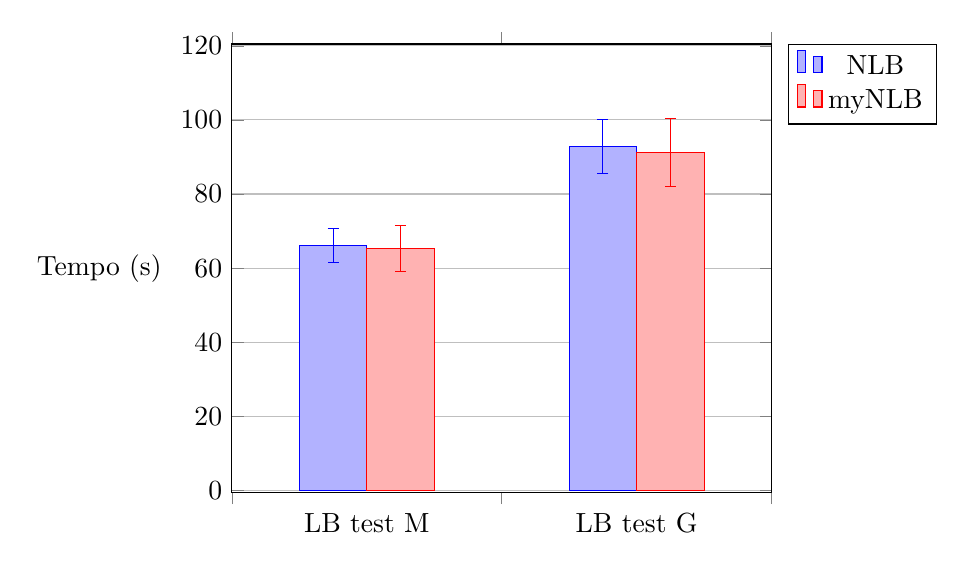
\begin{tikzpicture}
    \begin{axis}[
    legend pos=outer north east,
    enlargelimits={abs=0.5},
    ylabel style={rotate=-90},
    ylabel={Tempo (s)},
    ybar=0pt,
    ymajorgrids=true,
    bar width=0.25,
    ymin=0, ymax=120,
    xtick={0.5, 1.5, 2.5, 3.5 , 4.5},
    xticklabels={LB test M, LB test G, 5},
    x tick label as interval,
    ]
    
    \addplot+[error bars/.cd,
    y dir=both,y explicit]
    coordinates {
        (1, 66.21) +- (0.0, 4.59)
        (2, 92.76) +- (0.0, 7.29)};
    \addplot+[error bars/.cd,
    y dir=both,y explicit]
    coordinates {
        (1, 65.18) +- (0.0, 6.21)
        (2, 91.22) +- (0.0, 9.21)};
    
    \legend{NLB, myNLB}
    \end{axis}
    \end{tikzpicture}
    \caption[Comparação de tempos de balanceamento entre NeighborLB e myNeighborLB.] {Comparação de tempos de balanceamento entre NeighborLB e myNeighborLB. Os intervalos em cada barra representam o desvio padrão.}
    \label{fig:exec_times}
\end{figure}

As execuções realizadas com o \textit{benchmark LB test}, o balanceador NeighborLB e sua modificação para utilizar a Net Topo permitiram observar: (i) um sobrecusto de 3,5\% na inicialização do \charm, compensado largamente pelo ganho significativo na inicialização com XML; (ii) um sobrecusto abaixo do esperado no balanceamento, inclusive com menos custo que o do próprio \charm; e (iii) não houve um impacto negativo na qualidade do balanceamento, já que o algoritmo não foi modificado.
Estes resultados permitem afirmar o funcionamento desejado pela abstração.
Por outro lado, os experimentos realizados são bem limitados, pois observam uma escala reduzida de apenas duas máquinas e 12 PEs, o que inviabiliza assunções seguras em relação ao sobrecusto para outras escalas de aplicação.
Outra limitação dos experimentos é a avaliação de somente a função de vizinhança da abstração, não podendo, por exemplo, indicar o sobrecusto de se considerar uma topologia genérica em um cálculo de \textit{hops}.


% observar os ganhos com importação
% comentar as estruturas
%falar o escopo de avaliação limitada

\section{Avaliação de Desempenho}
\label{sec:bench}

Para observar o funcionamento da abstração em escalas diferentes, foi criado um gerador de topologias \fatt, \textit{mesh2D} e \textit{mesh3D} e observado os tempos de execução de 4 topologias geradas. 
Estes casos são apresentados na Seção~\ref{sec:bench:cases}.
A Tabela~\ref{tab:sizes_bench} apresenta as funcionalidades avaliadas e o número de execuções de cada uma. 
A função de inicialização é representada por \textit{init}, as de arquivamento e importação XML por \textit{save} e \textit{load}, respectivamente, e a de preenchimento do mecanismo de memoização por \textit{fill}.
Os cálculos de proximidade são detalhados logo antes de seus respectivos experimentos.

\setlength{\tabcolsep}{0.5em}
\begin{table}[!ht]
    \centering
    \begin{tabular}{l c}
        \toprule
        \textbf{Métodos} &    \textbf{Número de execuções} \\ \midrule
        \textit{init}, \textit{save} e \textit{fill} & $25$   \\ %\hline
        \textit{load} & $100$   \\ %\hline
        cálculos de proximidade & $200$ \\ \bottomrule
    \end{tabular}
    \caption[Número de execuções de cada função.]{Número de execuções de cada função testada. Um dos cálculos de proximidade foi executado 100 vezes em vez de 200.}
    \label{tab:sizes_bench}
\end{table}

A execução dos testes foi realizada na máquina Centauro, apresentada na Seção~\ref{subsec:ambiente}, utilizando um único núcleo e medindo o tempo através da biblioteca \textit{crono} de \textit{C++}.
Não foi utilizado um ambiente maior ou paralelo, pois o objetivo da execução era observar a variação de desempenho da estrutura em escalas diferentes.


% a velocidade não é questionada.
% valores de hop 1 e dist 1 não foram apresentados pois aprezentam valores de desvio padrão superior a 100%.

% definir cada coisa sendo testada, como vizinhança II
\subsection{Casos de Execução}
\label{sec:bench:cases}

Foram criados 4 casos de representações de topologias para a execução dos testes: uma \fatt com 7 níveis, nomeada de \textit{tree M}; uma \fatt de 10 níveis, representada como \textit{tree G}; uma \textit{mesh2D} de tamanho 16x16,  representada por \textit{mesh2D}; e uma \textit{mesh3D} simétrica de dimensão 8, nomeada \textit{mesh3D}.
Todas as topologias tiveram uma versão da abstração com memoização e outra sem. 
O número de máquinas e ligações de cada um dos casos de teste estão apresentados na Tabela~\ref{tab:sizes_topos}.
A coluna tamanho do arquivo XML e XML- representa o espaço em disco do arquivo XML gerado pela Net Topo com e sem memoização, respectivamente.
É possível observar que este tamanho não escala bem devido ao dispositivo de memoização, por ocupar espaço com complexidade $O(m^2)$ onde $m$ é o número de maquinas.

\setlength{\tabcolsep}{0.5em}
\begin{table}[!ht]
    \centering
    \begin{tabular}{l c c c c}
        \toprule
        \textbf{Caso} &    \textbf{Número de máquinas}  & \textbf{Número de ligações}  & \textbf{XML/M} & \textbf{XML} \\ \midrule
        \textit{tree M} & 127 & 126   & $0,32$  & $0,05$ \\ %\hline
        \textit{mesh2D} & 256 & 538   & $1,28$  & $0,12$  \\ %\hline
        \textit{mesh3D} & 512 & 1.344  & $5,06$  & $0,31$  \\ %\hline
        \textit{tree G} & 1.023 & 1.022 & $20,06$ & $0,42$  \\ \bottomrule
    \end{tabular}
    \caption[Tamanho das topologias]{Tamanho das abstrações criadas em número de máquinas, em número de ligações e em ocupação do arquivo XML em MB com e sem memoização, representado por XML/M e XML, respectivamente.}
    \label{tab:sizes_topos}
\end{table}

% execuções
% inicialização, save, fill: 25
% load, dist_2: 100
% hops, prox: 200
\subsection{Resultados}

Os resultados dos experimentos foram divididos em duas partes: (i) inicialização e serialização e (ii) cálculos de proximidade.
A primeira parte contempla os tempos de inicialização, arquivamento e importação XML de cada um dos casos.
A segunda compara os tempos de cálculo de proximidade, \hops e distância de cada um dos casos e do preenchimento do mecanismo de memoização nos casos que possuem memoização.
Para reduzir o desvio padrão e apresentar um resultado mais coerente, foram retirados da amostra casos discrepantes que ocorreram com baixa frequência (1\% ou menos) pois alteravam a média e o desvio padrão de maneira significante por serem valores de duas ordens de grandeza a mais.

\subsubsection{Inicialização e Serialização}

A Figura~\ref{fig:init_bench} apresenta o crescimento do tempo médio de inicialização, arquivamento e importação XML de cada um dos casos com o crescimento de número de máquinas.
As topologias \textit{tree M}, \textit{mesh2D}, \textit{mesh3D} e \textit{tree G} são representadas por $2^7$, $2^8$, $2^9$ e $2^{10}$ máquinas, respectivamente.
É possível observar que, quando sem memoização, os tempos de arquivar e importar crescem linearmente ou sublinearmente com a quantidade de máquinas.
Por outro lado é fácil observar que o mecanismo de memoização em forma de matriz não escala bem com o tamanho da topologia devido a sua natureza quadrática.
Isso se deve pelo fator da matriz de memoização representar metade de todas a ligações possíveis, que são mais de 524 mil no caso \textit{tree G}.

\begin{figure} [h]
\includegraphics[width=1.02\textwidth]{images/init_save_load.pdf}
\centering
\caption[Tempos de inicialização, arquivamento e importação XML.] {Crescimento dos tempo médio de inicialização (init), arquivamento (save) e importação XML (load) de cada um dos casos de teste. Os quadrados em azul são os casos com memoização e os triângulos em verde os casos sem memoização. }
\label{fig:init_bench}
\end{figure}

% \setlength{\tabcolsep}{0.5em}
% \begin{table}[!ht]
%     \centering
%     \begin{tabular}{| l | c | c | c |}
%         \toprule
%         \textbf{Caso} &    \textbf{\textit{init}} (ms) & \textbf{\textit{save}} (ms) & \textbf{\textit{load}} (ms)\\ \hline

%         \textit{tree M-}    & $1,06$ $(0,14)$   & $2,84$ $(0,24)$    & $3,89$ $(0,13)$  \\ \hline
%         \textit{tree M}     & $1,01$ $(0,01)$   & $16,46$ $(1,15)$     & $20,94$ $(0,06)$  \\ \hline
%         \textit{mesh2D-}    & $2,75$ $(0,18)$   & $6,98$ $(0,25)$     & $9,62$ $(0,19)$   \\ \hline
%         \textit{mesh2D}     & $2,63$ $(0,01)$   & $65,92$ $(3,64)$      & $82,38$ $(0,28)$   \\ \hline
%         \textit{mesh3D-}    & $5,97$ $(0,05)$   & $16,35$ $(0,16)$    & $22,47 $ $(1,01)$  \\ \hline
%         \textit{mesh3D}     & $6,95$ $(3,05)$  & $263,78$ $(10,31)$    & $322,76$ $(1,38)$   \\ \hline
%         \textit{tree G-}   & $7,75$ $(0,16)$   & $23,14$ $(0,83)$      & $29,82$ $(0,15)$   \\ \hline
%         \textit{tree G}    & $10,53$ $(5,56)$ & $1.068,07$ $(38,45)$   & $1.276,68$ $(8,04)$   \\ 
%         \bottomrule
%     \end{tabular}
%     \caption[Tempos de inicialização, arquivamento e importação XML.]{Tempos médios de inicialização, arquivamento e importação XML de cada um dos casos de teste. Desvio padrão entre parenteses.}
%     \label{tab:init_bench}
% \end{table}

\subsubsection{Cálculos de Proximidade}

A função de proximidade é um cálculo que avalia a proximidade entre dois PEs, observando se estão na mesma máquina ou não.
O tempo médio de um cálculo de proximidade foi entre 0,20 e 0,21 microssegundos em todos os casos de execução. 
O desvio padrão foi entre 0,04  e 0,06 microssegundos em todos os casos.
Foi observado que o cálculo de proximidade independe do tamanho da topologia e de ter ou não memoização, como era esperado.

O cálculo de distância avalia a latência entre duas máquinas da topologia.
Para avaliar a latência deste cálculo, foi agrupado o tempo de todos os cálculos de distância entre uma máquina e todas as máquinas a até dois \hops de distância dela. 
Este conjunto de distâncias calculadas foi denominado como ``distância II''.

O cálculo da distância II utiliza o mecanismo de memoização, e foram avaliados três cenários relativos a memoização: (i) inicialmente completa, (ii) inicialmente vazia e (iii) sem nenhum tipo de memoização.
A primeira contêm todas as informações de distância calculadas previamente.
A segunda inicia cada cálculo com a memoização inicialmente vazia, expandindo durante a execução de uma distância II.
O terceiro caso não utiliza nenhuma memoização e é utilizada para comparação.

A Tabela~\ref{tab:dist_comparison} apresenta os tempos médios de execução do preenchimento da matriz de memoização e dos três cenários de distância II.
A primeira coluna apresenta o tempo de preenchimento, que é o tempo o mecanismo de memoização através de cálculos de distância entre todos os nós.
A primeira linha de cada caso de execução indica a média dos tempos e a segunda linha o desvio padrão.

\setlength{\tabcolsep}{0.5em}
\begin{table}[!ht]
    \centering
    \begin{tabular}{l c c c c c}
        \toprule
        \textbf{Caso} & &   \textbf{Preenchimento} (ms)  & \textbf{Completa} ($\mu$s) & \textbf{Vazia} ($\mu$s) & \textbf{Sem memoização} ($\mu$s)\\ \midrule
        \multirow{2}{*}{\textit{tree M}}  & $\overline{x}$   & $75,70$   & $1,30$     & $11,32$    & $50,56$  \\
        & $\sigma$ & 0,98 & 0,04 & 4,68 & 13,15 \\ \hline
        \multirow{2}{*}{\textit{mesh2D}}  & $\overline{x}$   & $863,91$  & $2,69$     & $75,72$    & $210,42$   \\
        & $\sigma$ & 5,70 & 0,04 & 24,04 & 41,77 \\ \hline
        \multirow{2}{*}{\textit{mesh3D}}  & $\overline{x}$   & $4.880,94$   & $4,96$      & $214,90$   & $873,95$   \\
        & $\sigma$ & 19,03 & 0,35 & 21,12 & 77,39 \\ \hline
        \multirow{2}{*}{\textit{tree G}}  & $\overline{x}$  & $6.215,44$ & $1,40$    & $16,63$    & $39,49$   \\
        & $\sigma$ & 24,24 & 0,06 & 5,74 & 9,63 \\ \bottomrule
    \end{tabular}
    \caption[Tempos de cálculo de distância da vizinhança II.]{O tempo médio ($\overline{x}$) e o desvio padrão ($\sigma$) de preenchimento completo da matriz de memoização (primeira coluna), e tempo do cálculo de distância II de uma máquina com memoização completa (coluna II), inicialmente vazia (coluna III) ou inexistente (última coluna).}
    \label{tab:dist_comparison}
\end{table}

Todos os cálculos de distância têm um desvio padrão aumentado devido a variação do grau de cada máquina, sendo de 1 a 3 em uma \fatt, 2 a 4 numa \textit{mesh2D} e 3 a 6 em uma \textit{mesh3D}.
O desvio padrão maior no caso de memoização inicialmente vazia se deve ao fator dos cálculos oscilarem entre encontrar um valor armazenado e encontrar um valor novo.

Como o número de distâncias possíveis cresce quadraticamente com o número de máquinas, o tempo de preenchimento também cresce quadraticamente. Este crescimento é observável na Tabela~\ref{tab:dist_comparison}. 
Para que este tempo de preenchimento acelere a execução, é necessário que seu tempo seja pago por um número grande de cálculos de distância. 
No caso \textit{tree M}, por exemplo, são necessárias 6180 execuções, enquanto para \textit{tree G} são necessárias 125845 execuções.


Quando comparado o tempo de preenchimento da \textit{mesh3D} com da \textit{tree G}, este não cresceu tanto quando comparado com o crescimento entre \textit{mesh2D} e \textit{mesh3D}, por realizar um cálculo de distância com um grau médio menor.
Portanto o tempo de preenchimento da memoização cresce tanto com o número de máquinas na topologia quanto com o tempo de um cálculo de distância.
Com isso, a quantidade de execuções de distância para que o preenchimento valha a pela varia para cada topologia.

É possível observar um aumento no tempo conforme o grau da topologia aumenta, assim como uma melhoria entre a completa para a inicialmente vazia e outra melhoria entre a inicialmente vazia e a sem memoização.
A  melhoria no caso da inicialmente vazia se deve ao algoritmo de distância armazenar a distância de todos os visitados, conseguindo encontrar a distância de uma parte da vizinhança nas primeiras execuções e utilizá-la nas seguintes.

Na Tabela~\ref{tab:avg_dist_comparison} são apresentados os tempos médios de cada cálculo de distância individualmente feito na distância II, em vez de um agrupamento destes.
O desvio padrão se encontra altíssimo devido a vários fatores, como a variância do grau na topologia, a oscilação entre com e sem memoização e a imprecisão de relógio devido a magnitude sendo avaliada.
Devido a esta alta imprecisão os valores são estatisticamente equivalentes e por isso foi avaliado o tempo de vizinhanças, que não tinha tanta variância.
Ainda assim, é possível constatar um pequeno crescimento no cálculo de cada distância com o crescimento do grau.

\setlength{\tabcolsep}{0.5em}
\begin{table}[!ht]
    \centering
    \begin{tabular}{l c c c c}
        \toprule
        \textbf{Caso} & &   \textbf{Completa} & \textbf{Vazia} & \textbf{Sem memoização}\\ \midrule
        \multirow{2}{*}{\textit{tree M}}  & $\overline{x}$   & $0,24$      & $2,05$    & $9,16$  \\ 
        & $\sigma$ & 0,03 & 4,78 & $13,15$ \\ \hline
        \multirow{2}{*}{\textit{mesh2D}}  & $\overline{x}$  & $0,25$       & $6,94$    & $19,28$   \\ 
        & $\sigma$ & 0,04 & 14,05 & $21,74$\\ \hline
        \multirow{2}{*}{\textit{mesh3D}}  & $\overline{x}$   & $0,26$     & $11,62$   & $45,82$    \\ 
        & $\sigma$ & 0,35  & 23,11 & 27,66 \\ \hline
        \multirow{2}{*}{\textit{tree G}}  & $\overline{x}$   & $0,27$      & $3,2$    & $7,71$   \\
        & $\sigma$ & 0,06 & 5,7 & 5,6 \\
        \bottomrule
    \end{tabular}
    \caption[Tempo médio de um cálculo de distância.]{O tempo médio ($\overline{x}$) e desvio padrão ($\sigma$) de um cálculo de distância com memoização completa, inicialmente vazia ou inexistente.}
    \label{tab:avg_dist_comparison}
\end{table}

% hops varia com tamanho do grau médio, tree_7 e tree_10 tiveram valores menores e similares, enquanto mesh2D e 3D tiveram um aumento

O cálculo de \hops é outra métrica para avaliar proximidade entre duas máquinas, observando o número mínimo de \links entre uma máquina e outra.
Assim como o cálculo de distância, foi realizado um cálculo de \hops entre uma máquina e todas as máquinas a até dois \hops de distância, agrupando seus tempos num valor denominado de \hops II.
Esse agrupamento foi utilizado para estabilizar os valores, sendo que é possível encontrar a segunda vizinhança com \hops de maneira muito mais ágil.

Os tempos de \hops II são apresentados na Tabela~\ref{tab:dist_hop}, comparados com o tempo de distância II.
Assim como o cálculo de distância, os cálculo de \hops demonstrou um aumento no tempo de execução devido ao aumento do grau médio.
Não era esperado que os tempo de execução variasse com o número de máquinas, como ocorreu com a \textit{tree G}.

\setlength{\tabcolsep}{0.5em}
\begin{table}[!ht]
    \centering
    \begin{tabular}{l c c c c}
        \toprule
        \textbf{Caso}   &    & \textbf{Hops} ($\mu$s) &    \textbf{Distância} ($\mu$s) & \textbf{Sem memoização} ($\mu$s)\\ \midrule
        \multirow{2}{*}{\textit{tree M}} & $\overline{x}$    & $23,50$   & $11,32$  & $50,56$   \\ 
        & $\sigma$ & 6,36 & 4,68 & 13,15\\ \hline
        \multirow{2}{*}{\textit{mesh2D}} & $\overline{x}$    & $85,11$   & $75,72$ & $210,42$  \\
        & $\sigma$ & 13,39 & 24,04 & 41,77 \\ \hline
        \multirow{2}{*}{\textit{mesh3D}} & $\overline{x}$    & $534,50$  & $214,90$ & $873,95$  \\
        & $\sigma$ & 7,53 & 21,12 & 77,39 \\ \hline
        \multirow{2}{*}{\textit{tree G}} & $\overline{x}$     & $39,23$    & $16,63$ & $39,49$   \\
        & $\sigma$ & 2,46 & 5,74 & 9,63 \\ \bottomrule
    \end{tabular}
    \caption[Comparação entre hop e distância para vizinhança II.]{Comparação do tempo médio ($\overline{x}$) e desvio padrão ($\sigma$) de \hops II e distância II.}
    \label{tab:dist_hop}
\end{table}

Era esperado que o cálculo de \hops fosse mais rápido que o cálculo de distância em todos os casos mas, como não foi utilizado memoização para \hops, alguns casos de distância foram mais rápidos quando o grau médio foi elevado.
Isso se dá pelo armazenamento da distância de múltiplos vizinhos em um único cálculo de distância.
É possível observar que houve um acréscimo no tempo do cálculo de \hops, provavelmente devido a uma redução de localidade da cache.

Por fim, a Tabela~\ref{tab:memoi_worth} apresenta a aceleração do mecanismo de memoização na serialização e na distância II com memoização completa ou inicialmente vazia.
É importante que, mesmo com uma aceleração grande na distância, o tempo de preenchimento da memoização pode fazer com que não valha a pena.
No caso da \textit{tree G}, por exemplo, seria necessário em torno 164 mil execuções de distância II para que a redução no tempo comece a ser um benefício.

\setlength{\tabcolsep}{0.5em}
\begin{table}[!ht]
    \centering
    \begin{tabular}{l c c c c}
        \toprule
        \textbf{Caso}       & \textbf{\textit{save}} &    \textbf{\textit{load}} & \textbf{Vazia} & \textbf{Completa}\\ \midrule
        \textit{tree M}     & $0,172$   & $0,185$ & $4,46$ & $38,89 $ \\
        \textit{mesh2D}     & $0,105$   & $0,116$ & $2,77$ & $78,22$ \\
        \textit{mesh3D}     & $0,061$   & $0,069$ & $4,06$ & $176,00$  \\ 
        \textit{tree G}     & $0,021$   & $0,023$ & $2,37$ & $28,21$ \\ \bottomrule
    \end{tabular}
    \caption[Aceleração da memoização.]{Aceleração geradas pela memoização como matriz superior. As colunas \textit{save} e \textit{load} apresentam os atrasos no tempo médio de arquivamento e importação, respectivamente. As colunas \textit{Vazia} e \textit{Completa} apresentam a aceleração no tempo médio de distância II com memoização inicialmente vazia e completa, respectivamente. }
    \label{tab:memoi_worth}
\end{table}

Estes experimentos avaliaram o funcionamento da Net Topo em escalas diferentes e o impacto da memoização implementada.
Foi possível determinar que a memoização em forma de matriz não é escalável, causa um detrimento considerável no tempo para o arquivamento e importação e para que seu preenchimento valha a pena, seria necessário um número muito alto de execuções.
Apesar disso, ela gera uma aceleração considerável na execução do cálculo de distâncias de uma vizinhança, mesmo quando inicialmente vazia, mas este benefício depende do grau médio da topologia.
Em relação a escalabilidade da abstração, os tempos de inicialização, serialização, e proximidade escalaram de maneira adequada, mas os cálculos de distância e \hops cresceram ligeiramente com o número de máquinas, provavelmente devido a ocupação de memória.